% =========================================================================
% Capítulo 2: Cinética de la partícula
% Tema 01: Dinámica de la partícula
% Problema 12: Partícula en pista parabólica rotatoria
% Origen: Ayudantía 3, 2026
% =========================================================================
\subsubsection{Partícula en pista parabólica rotatoria}

Una partícula de masa $m$ se desliza sin fricción a lo largo de una pista en forma de parábola como se muestra en la \text{Figura \ref{fig:parabola_rotatoria}}. La ecuación que describe la geometría de la pista está dada por:
\[ y = \frac{r^2}{2a} \]
donde $a$ es una constante, $r$ es la distancia radial desde el eje vertical de simetría (punto $O$ al punto $B$), y $y$ es la distancia vertical desde el origen $O$ al punto $Q$. 

La partícula está unida a un resorte lineal de constante elástica $k$ y longitud natural $\ell_0$. El resorte se mantiene siempre alineado horizontalmente, conectando la partícula con un punto de unión libre de deslizarse a lo largo del eje vertical que pasa por el centro de la parábola. El sistema completo rota con una velocidad angular constante $\Omega$ alrededor de la dirección vertical. Considerando que la gravedad $\mathbf{g}$ actúa verticalmente hacia abajo, realice lo siguiente:

\begin{enumerate}
    \item Defina los marcos de referencia y sistemas de coordenadas adecuados para describir el movimiento en términos de la variable $r$.
    \item Analice la cinemática de la partícula, determinando el momento lineal y el momento angular respecto al punto $Q$.
    \item Analice la cinética de la partícula y determine la ecuación diferencial del movimiento en términos de la variable $r$.
\end{enumerate}

\begin{figure}[!ht]
    \centering
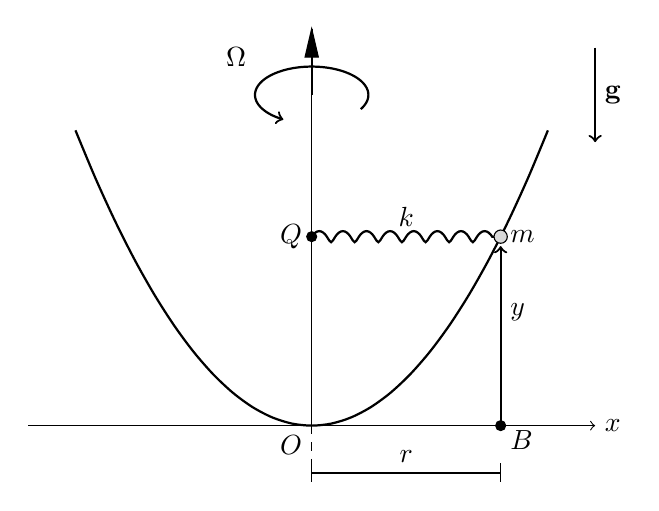
\begin{tikzpicture}[scale=1.2]
  % Axes
  \draw[->] (-3,0) -- (3,0) node[right] {$x$};
  \draw[-] (0,0) -- (0,4) ;

  % Origin
  \node[below left] at (0,0) {$O$};

  % Parabola
  \draw[domain=-2.5:2.5,smooth,variable=\x,thick] 
    plot ({\x},{0.5*\x*\x});

  % Dashed guides to Q
  \node[below, right] at (2,-0.15) {$B$};
    \filldraw[black] (2,0) circle (1.5pt);
  \draw[dashed] (0,0) -- (0,2) node[left] {$Q$};
    \filldraw[black] (0,2) circle (1.5pt);

  % Spring from Q to m
  \draw[decorate,decoration={coil,aspect=0.3, segment length=3mm, amplitude=2pt}, thick]
    (0,2) --node[midway,above] {$k$} (2,2);

  % Mass at end of spring
  \filldraw[fill=gray!30,draw=black] (2,2) circle (2pt);
  \node[right] at (2,2) {$m$};

  % Vertical arrow from parabola to mass: y
  \draw[->,thick] (2,0) -- (2,1.9);
  \node[right] at (2,1.2) {$y$};

  % Gravity arrow g
  \draw[->,thick] (3,4) -- (3,3);
  \node[right] at (3,3.5) {$\mathbf{g}$};

  \begin{scope}[shift={(0,3.5)}, rotate=0]
    \draw[->,thick] 
      plot[domain=-30:240,variable=\t,smooth,samples=100] 
      ({0.6*cos(\t)}, {0.3*sin(\t)});
    \node at (-0.8,0.4) {$\Omega$};
  \end{scope}
    % Axis stub and triangle tip
  \draw[thick] (0,3.5) -- (0,4.2);
  \draw[fill=black] (0,4.2) -- (-2pt,3.9) -- (2pt,3.9) -- cycle;

  %FLECHA r
  

\draw[-,dashed] (0,0)--(0,-0.5);
\draw[-,thick] (0,-0.5) -- node[midway, above] {$r$} (2,-0.5);
\draw (0,-0.4) -- (0,-0.6);
\draw (2,-0.4) -- (2,-0.6);

\end{tikzpicture}
    \caption{Diagrama de una partícula de masa $m$ en una pista parabólica rotatoria con vínculo elástico horizontal.}
    \label{fig:parabola_rotatoria}
\end{figure}

% --- SOLUCIÓN ---------------------------------------------------------------
\begin{solucion}{Partícula en pista parabólica rotatoria}

\textbf{Marcos de referencia y Sistemas de Coordenadas}\\
Lo primero, como en todo ejercicio, es definir los marcos de referencia.
\begin{itemize}
    \item $\mathcal{N}$: el suelo $\longrightarrow\{\vec{e}_x;\vec{e}_y;\vec{e}_z\}$
    \item $\mathcal{A}$: parábola $\longrightarrow\{\vec{e}_r;\vec{e}_\theta;\vec{e}_z\}$
\end{itemize}

\begin{center}
\begin{tikzpicture}[scale=0.8]
    \Polaresrtz{\Omega t}{e}{e}{azul}{myred}
    \node[above right] at (35:2) {$P$};
\end{tikzpicture}
\end{center}

\begin{equation*}
\begin{split}
    \vec{e}_r&=\cos(\Omega t)\vec{e}_x+\sin(\Omega t)\vec{e}_y\\
    \vec{e}_\theta&=-\sin(\Omega t)\vec{e}_x+\cos(\Omega t)\vec{e}_y\\
    \vec{e}_z&=\vec{e}_z
\end{split}
\end{equation*}

\subsubsection*{Cinemática de la partícula}
\textbf{Posición}\\
Como siempre, para obtener la velocidad de algún punto respecto a un marco inercial partimos por la posición; en este caso la de la masa $m$ es
$$\vec{r}_m=r\vec{e}_r+y\vec{e}_z$$

\textbf{Velocidad}\\
La velocidad es la derivada temporal de la posición:
$$\marc{\vec{v}_m}{N}=\der{\vec{r}_{m}}{N}=\der{(r\vec{e}_r+ y\vec{e}_z)}{N}=\dot r\vec{e}_r+r\der{\vec{e}_r}{N}{}+\dot y\vec{e}_z$$

\patotruco{No es necesario usar el teorema del transporte completo: usamos el trucazo (la demostración está en la Ayudantía 5). Como $\vec{e}_r$ y $\vec{e}_\theta$ giran solo en torno a $\vec{e}_z$ con velocidad angular $\Omega$, basta con $\dot{\vec{e}}_r=\Omega\vec{e}_\theta$ y $\dot{\vec{e}}_\theta=-\Omega\vec{e}_r$.}

Derivadas temporales de $\vec{e}_r$ y $\vec{e}_\theta$:
$$\transport{\vec{e}_r}{N}{A}=\Omega\vec{e}_z\times\vec{e}_r=\Omega\vec{e}_\theta$$
$$\transport{\vec{e}_\theta}{N}{A}=\Omega\vec{e}_z\times\vec{e}_\theta=-\Omega\vec{e}_r$$
y finalmente
$$\marc{\vec{v}_m}{N}=\dot r\vec{e}_r+r\Omega\vec{e}_\theta+\dot y\vec{e}_z$$

\textbf{Aceleración}\\
Al igual que antes, podemos simplemente derivar la velocidad:
% NOTA PARA REVISIÓN (agente B): el zip escribe -2 r' Omega e_theta; derivando la velocidad
% de arriba el signo es +2 r' Omega e_theta. Se deja tal cual (y arrastra el signo a N_b).
$$\marc{\vec{a}_m}{N}=\der{\marc{\vec{v}_m}{N}{}}{N}{}=\der{\left(\dot r\vec{e}_r+r\Omega\vec{e}_\theta+\dot y\vec{e}_z\right)}{N}{}=(\ddot{r}-r\Omega^2)\vec{e}_r-2\dot r\Omega\vec{e}_{\theta}+\ddot{y}\vec{e}_z$$
Obteniendo las derivadas de $y$ podemos reemplazar:
$$\dot y=\dfrac{r\dot r}{a}\qquad\ddot y=\dfrac{\dot r^2+r\ddot r}{a}$$

\textbf{Momento lineal y angular}\\
Para el cálculo del momento lineal hay que recordar cómo se define, y en este caso es
% NOTA PARA REVISIÓN (agente B): el zip escribe \dot y e_y en el momento lineal; por el contexto es \dot y e_z.
$$\marc{}{N}\vec{G}=m\cdot \marc{\vec{v}}{N}=m(\dot r\vec{e}_r+r\Omega\vec{e}_\theta+\dot y\vec{e}_y)$$
Por otro lado, el momento angular se tiene que calcular respecto a un punto; por ejemplo, podemos obtenerlo respecto al punto $Q$:
$$\marc{}{N}\vec{H}_Q=(\vec{r}_m-\vec{r}_Q)\times m(\vec{v}_m-\vec{v}_Q)$$
$$\marc{}{N}\vec{H}_Q=(r\vec{e}_r)\times m(\dot r\vec{e}_r+r\Omega\vec{e}_\theta)=mr^2\Omega\vec{e}_z$$

\subsubsection*{Cinética}
\textbf{Diagrama de cuerpo libre}\\
Cuando se hace análisis cinético hay que contar todas las cosas que uno elimina del problema y reemplazarlas por una fuerza; en este caso, cuando nos quedamos solo con la partícula:

\begin{center}
\begin{tikzpicture}[>=Latex, scale=1.0]
    % --- PARÁMETROS ---
    \def\a{1.5}       % constante de la parábola [u]
    \def\rp{1.8}      % posición radial de la partícula [u]

    % --- EJE Y PARÁBOLA ---
    \draw[->, thin] (0,-0.2) -- (0,3.1) node[above] {$\vec{e}_z$};
    \draw[thick, domain=0:2.6, smooth, samples=40, variable=\x] plot ({\x},{\x*\x/(2*\a)});
    \draw[->, thin] (0,0) -- (3.0,0) node[right] {$\vec{e}_r$};

    % --- PARTÍCULA Y BASE TNB ---
    \pgfmathsetmacro{\yp}{\rp*\rp/(2*\a)}
    \pgfmathsetmacro{\nrm}{sqrt(1+(\rp/\a)^2)}
    \coordinate (M) at (\rp,\yp);
    \draw[dashed, gray] (M) -- (0,\yp);
    \draw[dashed, gray] (M) -- (\rp,0) node[below] {\textcolor{gray}{$r$}};
    \draw[->, ultra thick, myred] (M) -- ++({1/\nrm},{(\rp/\a)/\nrm}) node[right] {$\vec{e}_t$};
    \draw[->, ultra thick, azul] (M) -- ++({-(\rp/\a)/\nrm},{1/\nrm}) node[above] {$\vec{e}_n$};
    \draw (M) ++(0.3,-0.3) circle (0.1); \draw ($(M)+(0.3,-0.3)+(-0.07,-0.07)$) -- ++(0.14,0.14); \draw ($(M)+(0.3,-0.3)+(-0.07,0.07)$) -- ++(0.14,-0.14);
    \node[green!50!black, right] at ($(M)+(0.4,-0.3)$) {$\vec{e}_b=\vec{e}_\theta$};
    \shadedraw[ball color=gray!30] (M) circle (3pt);
\end{tikzpicture}
\hspace{1cm}
\begin{tikzpicture}[>=Latex, scale=1.0]
    \def\a{1.5}
    \def\rp{1.8}
    \draw[->, thin] (0,-0.2) -- (0,3.1) node[above] {$\vec{e}_z$};
    \draw[thick, domain=0:2.6, smooth, samples=40, variable=\x] plot ({\x},{\x*\x/(2*\a)});
    \pgfmathsetmacro{\yp}{\rp*\rp/(2*\a)}
    \pgfmathsetmacro{\nrm}{sqrt(1+(\rp/\a)^2)}
    \coordinate (M) at (\rp,\yp);
    \draw[decoration={coil, aspect=0.4, segment length=3pt, amplitude=2.5pt}, decorate, thick] (M) -- (0,\yp);
    \node[above] at (0.9,\yp+0.1) {$K$};
    \draw[->, ultra thick, myred] (M) -- ++(-0.9,0) node[below left] {$\vec{F}_s$};
    \draw[->, ultra thick, myred] (M) -- ++(0,-1.0) node[below] {$\vec{F}_g$};
    \draw[->, ultra thick, azul] (M) -- ++({-(\rp/\a)/\nrm*1.0},{1/\nrm*1.0}) node[above] {$\vec{N}_n$};
    \draw (M) ++(0.3,-0.3) circle (0.1); \draw ($(M)+(0.3,-0.3)+(-0.07,-0.07)$) -- ++(0.14,0.14); \draw ($(M)+(0.3,-0.3)+(-0.07,0.07)$) -- ++(0.14,-0.14);
    \node[green!50!black, right] at ($(M)+(0.4,-0.3)$) {$\vec{N}_b$};
    \shadedraw[ball color=gray!30] (M) circle (3pt);
\end{tikzpicture}
\end{center}

$\vec{F}_g$, la fuerza de gravedad, es el reemplazo de sacar la ``tierra'' y es $\vec{F}_g=m\vec{g}=-mg\vec{e}_z$.\\
$\vec{F}_s$ es la fuerza que reemplaza al resorte, se escribe como $\vec{F}_s=-k(r-\ell_0)\vec{u}$, donde $\vec{u}=\dfrac{\vec{r}_m-\vec{r}_Q}{\|\vec{r}_m-\vec{r}_Q\|}=\vec{e}_r$.\\
Finalmente tenemos las normales. Se preguntarán por qué hay 2: la normal es una sola, lo que ocurre es que no conocemos ni la dirección ni la magnitud de la normal. Lo que sí sabemos es que, respecto a la parábola, la partícula se mueve solamente en la dirección tangente (esto ocurre porque la parábola restringe el movimiento). Pueden pensarlo como que la parábola es la intersección de dos superficies y por ende tiene ``2'' normales, pero en realidad es una, y su dirección está siempre en las direcciones normal y binormal de la curva (vista por un observador en la curva). No podría ser la tangente porque por ahí se mueve la partícula.
$$\vec{N}=N_b\vec{e}_b+N_n\vec{e}_n$$
Entonces partimos calculando la base intrínseca en alguna base conocida, como la cilíndrica:
$$\vec{e}_t=\dfrac{\marc{\vec{v}_m}{A}}{\|\marc{\vec{v}_m}{A}\|}\quad\longrightarrow\quad\marc{\vec{v}_m}{A}=\der{(r\vec{e}_r+y\vec{e}_z)}{A}{}=\dot r\vec{e}_r+ \dfrac{r\dot r}{a} \vec{e}_z\quad\longrightarrow\quad\vec{e}_t=\dfrac{\dot r\vec{e}_r+\left(\dfrac{r\dot r}{a}\right)\vec{e}_z}{|\dot r|\sqrt{1+(r/a)^2}}$$
Antes de obtener $\vec{e}_n$ nos podemos dar cuenta de que, físicamente, el vector $\vec{e}_b$ tiene que ser la normal del plano que contiene a la parábola; mejor dicho, tiene que ser perpendicular a la parábola y, con regla de la mano derecha, se llega a que $\vec{e}_b=\vec{e}_\theta$. Entonces, con el producto cruz $\vec{e}_b\times\vec{e}_t=\vec{e}_n$:
$$\vec{e}_n=\vec{e}_\theta\times\dfrac{\dot r\vec{e}_r+\left(\dfrac{r\dot r}{a}\right)\vec{e}_z}{|\dot r|\sqrt{1+(r/a)^2}}=\dfrac{\dot r\vec{e}_z-\left(\dfrac{r\dot r}{a}\right)\vec{e}_r}{|\dot r|\sqrt{1+(r/a)^2}}$$
Por simplicidad cancelaremos $\dot r/|\dot r|=1$, y el signo que le corresponde irá con la magnitud de la normal.
\begin{equation*}
\begin{split}
    \vec{e}_t&=\dfrac{\vec{e}_r+\left(\dfrac{r}{a}\right)\vec{e}_z}{\sqrt{1+(r/a)^2}}\\
    \vec{e}_n&=\dfrac{\vec{e}_z-\left(\dfrac{r}{a}\right)\vec{e}_r}{\sqrt{1+(r/a)^2}}\\
    \vec{e}_b&=\vec{e}_\theta
\end{split}
\end{equation*}

\textbf{Ecuación diferencial}\\
Ahora es cuando aplicamos la segunda ley de Newton:
$$\sum\vec{F}_{ext}=m\marc{\vec{a}_m}{N}$$
$$-mg\vec{e}_z-k(r-\ell_0)\vec{e}_r+N_b\vec{e}_b+N_n\vec{e}_n=m\left((\ddot{r}-r\Omega^2)\vec{e}_r-2\dot r\Omega\vec{e}_{\theta}+\dfrac{\dot r^2+r\ddot r}{a}\vec{e}_z\right)$$
Ahora tenemos dos maneras de encontrar la ecuación que rige el movimiento de $r$. La primera, y la más común, es pasar de la ecuación vectorial a 3 ecuaciones escalares. Lo que se dice es ``masa por aceleración en $\vec{e}_r$ es igual a suma de fuerzas en $\vec{e}_r$'', pero lo que matemáticamente se hace en realidad es esto:
\begin{equation*}
\begin{split}
   \vec{e}_r\cdot \sum\vec{F}_{ext}&=\vec{e}_r\cdot m\marc{\vec{a}_m}{N}\\
   \vec{e}_\theta\cdot \sum\vec{F}_{ext}&=\vec{e}_\theta\cdot m\marc{\vec{a}_m}{N}\\
   \vec{e}_z \cdot \sum\vec{F}_{ext}&=\vec{e}_z\cdot m\marc{\vec{a}_m}{N}
\end{split}
\end{equation*}
y el sistema de 3 ecuaciones se ve así:
% NOTA PARA REVISIÓN (agente B): en el zip la primera ecuación trae (1+(r/a)^2) en vez de su raíz,
% (r - x_0) en vez de (r - l_0) y +k donde por el DCL corresponde -k. Se deja tal cual.
\begin{align*}
- \left[ \frac{N_n \, (r/a)}{1 + (r/a)^2} \right] + k (r - x_0) &= m \left( \ddot{r} - r \Omega^2 \right) \\[1em]
\left[ \frac{N_n}{\sqrt{1 + (r/a)^2}} - mg \right] &= \frac{m}{a} \left( \dot{r}^2 + r \ddot{r} \right) \\[1em]
N_b &= -2m \dot{r} \Omega
\end{align*}
Lo que buscamos en realidad es algo del estilo $\ddot r=f(\dot r,r,\Omega,\dots)$ con todas cosas conocidas (las derivadas pasadas de las variables se consideran conocidas). Para eso sería una lata tener que andar despejando y multiplicando para eliminar las normales que nos molestan.

\patotruco{Otro método: encontrar una dirección donde se vayan las cosas que nos molestan. Lo único que molesta aquí son las normales, y la única dirección perpendicular a ambas es $\vec{e}_t$. Como solo importa la dirección, multiplicamos por $A=\sqrt{1+(r/a)^2}$ para proyectar en $A\,\vec{e}_t$.}

\begin{align*}
(\vec{e}_r+(r/a)\vec{e}_z)\cdot(-mg\vec{e}_z-k(r-\ell_0)\vec{e}_r)&=A\vec{e}_t\cdot m\left((\ddot{r}-r\Omega^2)\vec{e}_r-2\dot r\Omega\vec{e}_{\theta}+\dfrac{\dot r^2+r\ddot r}{a}\vec{e}_z\right)\\
-mg\dfrac{r}{a}-k(r-\ell_0)&= m\left((\ddot{r}-r\Omega^2)+\left(\dfrac{r}{a}\right)\dfrac{\dot r^2+r\ddot r}{a}\right)
\end{align*}
Distribuimos y expandimos el segundo término del lado derecho:
$$- mg \frac{r}{a} - k(r - \ell_0) = m\left( \ddot{r} - r\Omega^2 + \frac{r}{a^2}(\dot{r}^2 + r\ddot{r}) \right)= m\left( \ddot{r} - r\Omega^2 + \frac{r}{a^2} \dot{r}^2 + \frac{r^2}{a^2} \ddot{r} \right)$$
Agrupamos los términos con $\ddot{r}$:
$$- mg \frac{r}{a} - k(r - \ell_0) = m\left( \left(1 + \frac{r^2}{a^2} \right)\ddot{r} - r\Omega^2 + \frac{r}{a^2} \dot{r}^2 \right)$$
Dividimos todo entre $m$ y pasamos los términos al otro lado:
$$\frac{- mg \frac{r}{a} - k(r - \ell_0)}{m} + r\Omega^2 - \frac{r}{a^2} \dot{r}^2 = \left(1 + \frac{r^2}{a^2} \right)\ddot{r}$$
Finalmente, despejamos $\ddot{r}$:
\respuesta{$\displaystyle \ddot{r} = \frac{ -\dfrac{g r}{a} - \dfrac{k}{m}(r - \ell_0) + r\Omega^2 - \dfrac{r}{a^2} \dot{r}^2 }{ 1 + \dfrac{r^2}{a^2} }$}

\end{solucion}
